
The last 12 months have been devoted to understanding the mathematical and biological background for alignment based comparative genomics techniques as described in detail above. Some preliminary work has been done using Change Point~\cite{keith2006segmenting} that was presented in a poster at SMB 2018. My primary output in this time has been code written for the purposes of model selection and analysis relating to Change Point. A sample of the preliminary work can be seen in Figure~\ref{fig:wigglel}; this was presented in a poster at the SMB conference in 2018, where I was a recipient of a travel grant.

\begin{figure}[H]
    \centering
    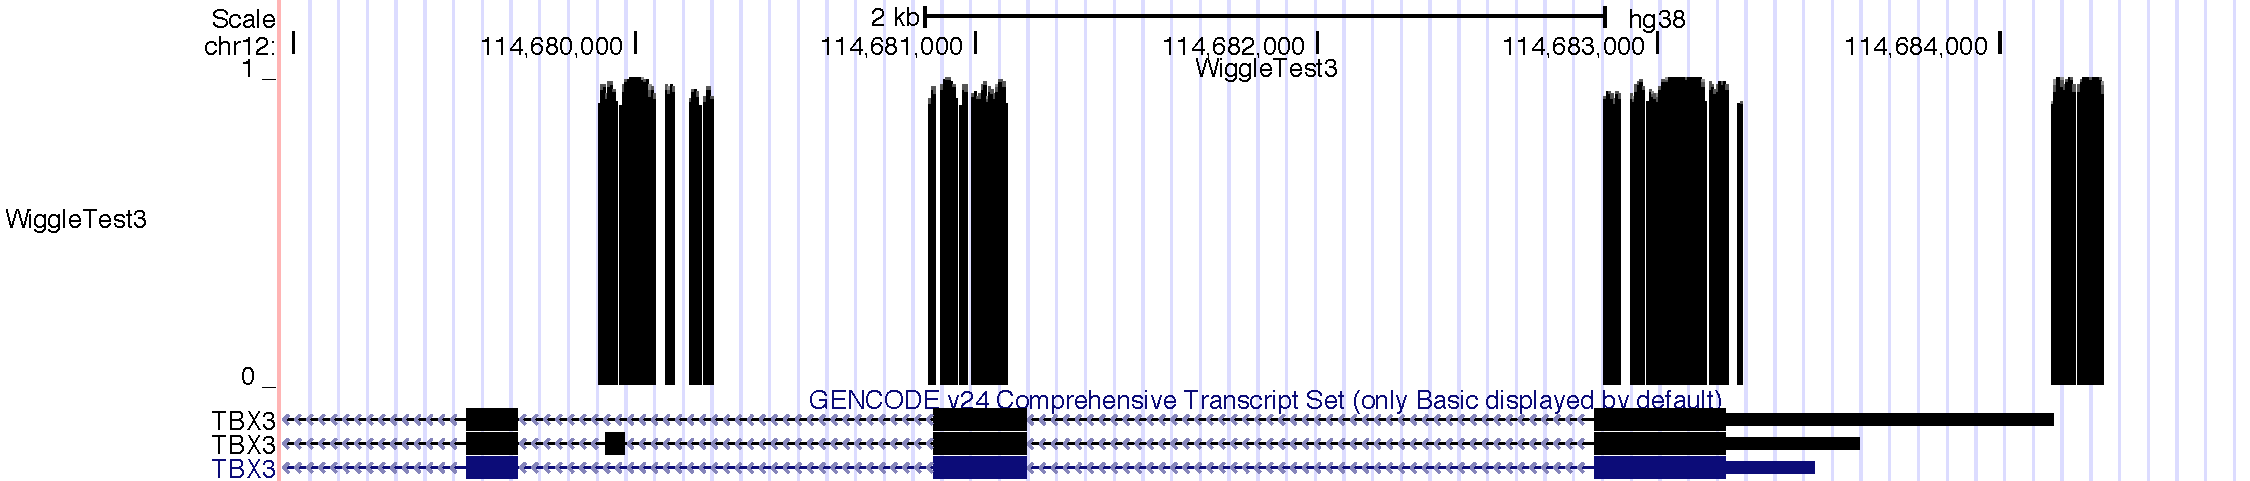
\includegraphics[width = \textwidth]{WiggleTrack1.pdf}
    \caption{A sample of the output generated by work dong up to this point with Change Point. The bars represent sequence positions that belong to a particular segment class with $\geq$ 0.9 probability and are at least 100 nucleotides in length.}
    \label{fig:wigglel}
\end{figure}

This analysis was only applied to a small region surrounding one gene. However, in the process of applying this methodology, I have learned a lot about some of the strengths and weaknesses associated with alignment based approaches that rely heavily on conservation as well as a large amount about the background biology and the underlying processes relating to gene expression. 

A large amount of time was devoted to:
  \begin{itemize}
        \item learning the background biology, the computing languages; Python, R and C++.
        \item learning advanced statistical theory, such as hierarchical bayesian modelling, MCMC techniques and measure theory.
        \item writing scripts for model selection and analysis for change point output.
        \item Attending workshops and conferences: AMSI Bioinfosummer (2017), SMB (2018), Software Carpentry (2017).
    \end{itemize}
    